\chapter{Mise en place d'un modèle de formation et d'évolution stellaire}
\label{sec:etoiles}

Dans les parties précédentes nous avons rapidement présenté quelles étaient les différentes physiques à l’œuvre dans les simulations de la réionisation et la façon dont elles sont modélisées numériquement.
Il manque encore une composante essentielle au problème qui est la modélisation des sources de rayonnement ionisant.
L'objectif de cette section est d'exposer le modèle de sources que j'ai développé, implémenté et calibré.
Comme nous avons vu en introduction (cf section \ref{sec:introreio}), il existe deux types de sources, les étoiles et les quasars.
Dans la suite de cette étude, je n'ai considéré que la partie stellaire sans me préoccuper des quasars.
Nous allons définir les différentes phase de la vie d'une étoile, et ses différentes évolutions possible.
Nous verrons comment les contraintes imposées par les échelles cosmologique que l'on cherche à étudier vont imposer certains choix au niveau numérique.
Une attention particulière sera mise sur la modélisation des supernovae, puisque une étude comparative entre deux modèles d'injection d'énergie suivra.
Lors de cette comparaison, il s'est avéré que dans nos modèles, les supernovæ étaient capable de réguler le \ac{SFR}, sans changer l'histoire de la réionisation.

%\section{Les différentes phases de la vie d'une étoile}
%
%L'objectif est ici de définir les différentes phases de la vie d'une étoile.
%Nous allons aborder sa naissance, sa vie et sa mort de manière générale dans un premier temps.
%Et nous verrons ensuite l'implémentation de ces trois phases dans EMMA.

%\section{Modèle sous grille et population stellaire}

\section{Considérations de résolution}
%En fonction des echelles de travail, nous considererons soit les etoiles individuelles soit une population stellaire.

Une des difficulté majeurs dans les simulations de la réionisation, est l'impossibilité d'obtenir des résolutions suffisante pour suivre la formation des sources de radiation individuellement, tout en simulant un volume suffisamment important.
%Il existe toujours ce conflit en réionisation entre simuler des grands volume, et obtenir la meilleur résolution possible.
Actuellement les simulations capables de suivre un volume d'Univers de l'ordre de $(100Mpc)^3$ atteignent un résolution de l'ordre du kilo-parsec.
Or les échelles de formation stellaire sont de l'ordre de l'unité astronomique, soit un facteur $\approx 10^8$ plus petit.
Il est donc actuellement impossible de résoudre les deux cotés du spectre d'échelles spatiales.
%de suivre la formation des étoiles individuellement.
Il est nécessaire de créer un modèle qui va tenter de prendre en compte au mieux la physique non résolue.
Ce type de modèle est appelé modèle \textit{sous grille}.
Dans le cas présent le modèle sous grille consiste à transformer une partie du gaz en particule stellaire, cette particule ne représentant pas une étoiles mais une population stellaire de manière statistique.
%On appelle ces particules des particules puits.
Toute la difficulté du modèle de formation stellaire sera de déterminer la façon dont est réalisée cette conversion.
Malgré tout, nous verrons qu'il est possible d'obtenir un modèle statistiquement viable à grandes échelles assez facilement.

% Un second type de modèle intervient au moment de l'explosion en supernovae.
% Les processus de diffusion de l'énergie libérée aux échelles plus petite que la grille sont complexe et il en résulte une série de paramètres libres assez conséquente.

%lien entre les différents solveurs en fonction du stade évolutif
%Les étoiles se trouvent aux centre de la simulation.
%En effet, créer une étoiles consiste a transformer une partie du gaz en particule.
%Cette particule sera ensuite gérée par le solveur Ncorps, et servira de source au solveur radiatif.
%Puis a la fin de sa vie, l'étoile va injecter de l'énergie dans le solveur hydrodynamique.
%Une particule stellaire va donc devoir interagir avec tout les solveurs du code.

%Seul la partie du spectre capable de ioniser l'hydrogène est considérée. E>13.6eV



\section{La formation stellaire}

\subsection{Naissance}

%lien avec la densité\\
%Formation dans l'H moléculaire mais pas dans les simu

Les étoiles se forment au sein de nuage de gaz, par effondrement gravitationnel.
Si les conditions sont réunies, cet effondrement ne s'arrête quand les réactions thermonucléaire s'enclenchent et que le gaz forme une étoile.
En première approximation, un nuage de gaz s'effondre, si le temps de chute libre : 
\begin{equation}
t_{ff} =  \sqrt{\frac{3\pi}{32G\rho_g}} \propto \frac{1}{\sqrt{G \rho}},
\label{eq:tff}
\end{equation}
est supérieur au temps de réaction à une perturbation.
Considérant que cette perturbation est d'origine mécanique, le temps de réaction sera équivalent au temps de traversée du nuage par une onde sonore :
 \begin{equation}
t_{sound} = \frac{R}{C_s},
\end{equation}
avec $R$ la taille du nuage et $C_s$ la vitesse du son dans ce nuage.
Si le temps de réaction est plus long que le temps de chute libre
\begin{equation}
t_{ff} < t_{sound},
\end{equation}
alors le milieu n'a pas le temps de résister et le nuage s'effondre sur lui même.

$t_{ff}$ fait intervenir la densité, plus le milieu est dense plus il aura tendance à s'effondrer sur lui même.
Et de l'autre coté intervient aussi la vitesse du son $C_s$, elle même dépendante de la température $C_s \propto \sqrt{T}$.
Plus le gaz sera chaud, plus le nuage va résister a son effondrement.
%\subsection{Population III}
%tres peu de ligne de refroisdissment
%étoiles plus grosse
% temps de vie court
A haut redshift, au moment de l'apparition des premières étoiles, les métaux étaient très peu disponible (voir :\ref{sec:nucleosynthese_primordiale}).
De ce fait, le gaz disposait de relativement peu de possibilité de refroidissement, menant à une température plus élevée.
Les étoiles primordiales devaient donc être plus grosses que les étoiles de notre voisinage (plus de $100M_\odot$).
Ce type d'étoiles est appelées étoiles de population III ou popIII.

%La nucléosynthèse primordiale a créer peu de métaux. 
%A haut redshift, les metaux etaient peu disponible.
%les métaux permettent une meilleur emmission radiative, et donc un meilleur refroidissent.
%si le refroidissment est meilleur, l'equilibre hydrostatique penche an faveur de plus grosse étoiles.
%POPIII, IMF top Heavy, étoiles  primordiales
%
%plus un étoiles est grosse, plus son spectre sera énergétique et plus la portion de spectre ionisant sera important.



L'objectif de cette section est de présenter le modèle de formation stellaire que j'ai implémenté dans EMMA.
Dans ce modèle, la formation stellaire a lieu en trois temps.
Il faut d'abord localiser les régions de formation, puis calculer la quantité d'étoile à former, et enfin former les particules.
 
\subsection{Localisation des zones de formation stellaire}

Il est admis que les étoiles se forment dans les nuages d'hydrogène moléculaire (voir eg \cite{krumholz_universal_2012}).
Ces nuages se trouvent eux même dans des zones suffisamment denses pour que des molécules puissent se former.
En pratique dans EMMA, la physique de l'hydrogène moléculaire n'est pas encore prise en compte, et les zones autorisées à former des étoiles sont localisées à l'aide d'un seuil en densité.
Toutes les cellules plus dense qu'un certain seuil sont autorisées à créer des particules stellaire.

%Seuil en densité \\
\begin{equation}
	flag = 
  \begin{cases}
      True, & \text{if } \rho > \rho_{thresh}\\
      False,              & \text{otherwise}
  \end{cases}
\end{equation} 

Cette densité de seuil $\rho_{thresh}$ peux être définie arbitrairement, et comme toute densité, elle est dépendante de la résolution.
De plus il en possible de définir une densité en unité physique ou en unité commobile (voir section \ref{sec:supercomobil}).
Un seuil en densité physique sera plus représentatif de se qui se passe réellement.
Mais à haut redshift, la densité était importante en tout points, et un seuil en unité comobile est utile pour limiter l'apparition des premières étoiles à un redshift donné.
En pratique on pourra définir ces deux seuils, et le seuil final sera le plus contraignant des deux.

%TODO figure du seuil en fonction du redshift

\begin{equation}
	\rho_{thresh} = max\left(  \delta_{in} \bar{\rho}, \rho_{in} a^3 \right)
\end{equation} 

ou $\delta_{in}$ et $\rho_{in}$  sont respectivement les paramètres de surdensité et de densité physique.
$\delta_{in}$ est exprimé en unité comobile et est donc constant dans le temps en unités du code,
 $\rho_{in}$ est exprimé en unité physique (en atome par mètre cube), sa valeur évolue dans le temps du point de vue des unités du code (cf section \ref{sec:supercomobil}).

% determination de la valeur de 55\\ 
%TODO quells valeurs sont prisent et pourquoi?

\subsection{La loi de schmidt-kennicut}
\label{sec:schmidt-kennicut}
 %conversion densité surfacique vers densité 3D\\
%rho 1.5\\
%temps de free fall\\

Maintenant que nous avons définis où former des étoiles, il nous faut calculer la quantité à former.
La loi de Schmidt \citep{1959ApJ...129..243S}  est une loi observationnelle qui lie la densité surfacique de gaz dans les galaxies au taux de formation stellaire (\ac{SFR}) dans cette galaxie.
\cite{1998ApJ...498..541K} a utilisé un modèle de galaxie pour dé-projeter la densité surfacique observée et ainsi déterminer une loi qui lie le \ac{SFR} à la densité volumique de gaz.
Cette loi a la forme:
\begin{equation}
SFR \propto \rho ^{\alpha},
\end{equation}
avec $\alpha \approx 1.4 \pm 0.15$

Le taux de formation stellaire s'exprime généralement en $M_\odot \cdot cMpc^{-3} \cdot yr^{-1}$  
Ce qui est homogène à une densité divisé par un temps.
En pratique divisera $\rho_g$ la densité locale de gaz par le temps de chute libre (equation \ref{eq:tff}), qui est en théorie le temps nécessaire à un nuage de gaz pour s'effondrer si il n'y avait aucune résistance.
Au final, le \ac{SFR} prend la forme:
\begin{equation}
	SFR = \epsilon_{sf} \frac{\rho_g}{t_{ff}} \propto \rho_g^{1.5}
    \label{eq_sfr}
\end{equation}
avec  $\epsilon_{sf}$ le paramètre d'efficacité de formation stellaire.
Observationellement, $\epsilon_{sf}$  est de l'ordre du \%. %TODO ref
Ce qui signifie que la formation stellaire est relativement inefficace.
Il est également possible de considérer le temps caractéristique de formation stellaire:
\begin{equation}
t_{sf} =  \frac{t_{ff}}{ \epsilon_{sf} },
\end{equation}
qui est de l'ordre de quelques milliards d'années.



\subsection{Implémentation}

A partir du taux de formation, on obtient la masse de gaz à convertir en étoiles dans chaque cellule en multipliant par $dv$ le volume de la cellule en question et $dt$ le pas de temps entre deux passage dans la fonction de formation stellaire:
\begin{equation}
	M_{star} = SFR \cdot dv \cdot dt .
\end{equation}

%resolution en masse\\
Nous avons donc à ce stade la masse totale de gaz à convertir en étoile.
Il devient rapidement coûteux de générer pour chaque cellule éligible, et à chaque pas de temps, une nouvelles particule stellaire (le nombre de particule peux rapidement exploser).
Nous adoptons une approche probabiliste.
Nous définissons une masse d'étoiles $m_{star}$ qui correspondra à notre "quanta stellaire".
Toutes les étoiles aurons donc la même masse et cette masse est calculée d'une manière comparable à celle d'une particule de matière noire.
La masse d'une étoile correspond à la masse moyenne de gaz dans une cellules d'un certain niveau :
\begin{equation}
 m_{star} = M_{DM} \frac{\Omega_b}{\Omega_m}\cdot 2^{-3L},
\end{equation}
où $L$ peux varier du niveau de base à niveau plusieurs niveaux raffinés.

%TODO cite RAMSES
Le nombre de quanta à ajouter est ensuite tiré aléatoirement dans une loi de Poisson \citep{rasera_history_2006}.
\begin{equation}
	P(N) = \frac{\lambda^N}{N!} e^{-\lambda}
\end{equation}

Où $\lambda$ correspond au nombre de particules moyen à créer dans la cellule :
\begin{equation}
\lambda = \frac{ M_{star}}{m_{star}}
\end{equation}
On obtiendra au final $N_{star}$ le nombre de quanta de masse d'étoiles à créer.
Étant donné le grand nombre de tirage cette loi est en moyenne valide.

En pratique j'ai implémenté deux méthodes de transformations.
Si  $N_{star}>1$ il est possible de créer : 
\begin{itemize}
\item  $N_{star}$ particules aillant chacune une masse  $m_{star}$.
\item une seule particule de masse  $N_{star} \cdot m_{star}$.
\end{itemize}

Dans le premier cas le nombre de particules sera plus élevée et la résolution stellaire meilleure, mais en contrepartie le coût numérique sera plus important.
Le choix de la méthode est laissé à l'utilisateur et dépend de la situation.

%En pratique la création d'une particule stellaire consistera a 
%\begin{itemize}
%\item prendre dans la réserve, une nouvelle particule %un maillon de la liste chainée
%\item ajouter ce nouveau maillons a la liste chainée de particule de la cellule.
%\item initialiser cette nouvelle particule avec : 
%\begin{itemize}
%\item un état
%\item un temps de création
%\item une vitesse 
%\item une masse
%\item un identifiant
%\end{itemize}
%\end{itemize}

%TODO resolution masse stellaire
%TODO conservation de la masse

En pratique la création d'une particule stellaire consistera à prendre une nouvelle particule vierge dans la réserve (cf section \ref{sec:PART}), ajouter ce nouveau maillons à la liste chaînée de particule de la cellule et initialiser cette nouvelle particule.

On associera un instant de création à la particule stellaire et non un age, ceci permet de ne pas avoir à remettre à jour cette valeur à chaque pas de temps.
Pendant les analyses post-simulations, on prendra garde à définir l'age des étoiles comme étant l'instant associé au snapshot courant moins l'instant de création de la particule.

Les étoiles créées auront une vitesse correspondant à la vitesse du gaz au moment de leurs création.
Pour éviter les effets de "collier", à cette vitesse sera ajoutée une composante aléatoire, aillant une direction aléatoire et une amplitude aléatoirement comprise entre $\pm c_s$ la vitesse du son dans la cellule \citep{rasera_history_2006}.

Il est utile d'associer un identifiant unique aux nouvelles particules pour pouvoir suivre leurs évolutions et les retrouver entre les différentes sorties.
La technique la plus simple est d'associer la valeur d'un entier que l'on incrémente à chaque création d'une nouvelle particule.
Du fait de la parallélisation cette incrémentation demande des communications à chaque création de particule.
Pour minimiser les communications, la pratique retenue consiste à former toutes les particules de toutes les processus, en leur assignant un identifiant caractéristique (eg -1) et d'assigner les identifiants finaux dans un second temps.
Une fois les particules créées, chaque processus compte son nombre de nouvelles particules et le transmet aux autres, ce qui permet d'allouer une plage d'identifiants par processus, et ainsi allouer les identifiants finaux.


%\begin{figure}
%        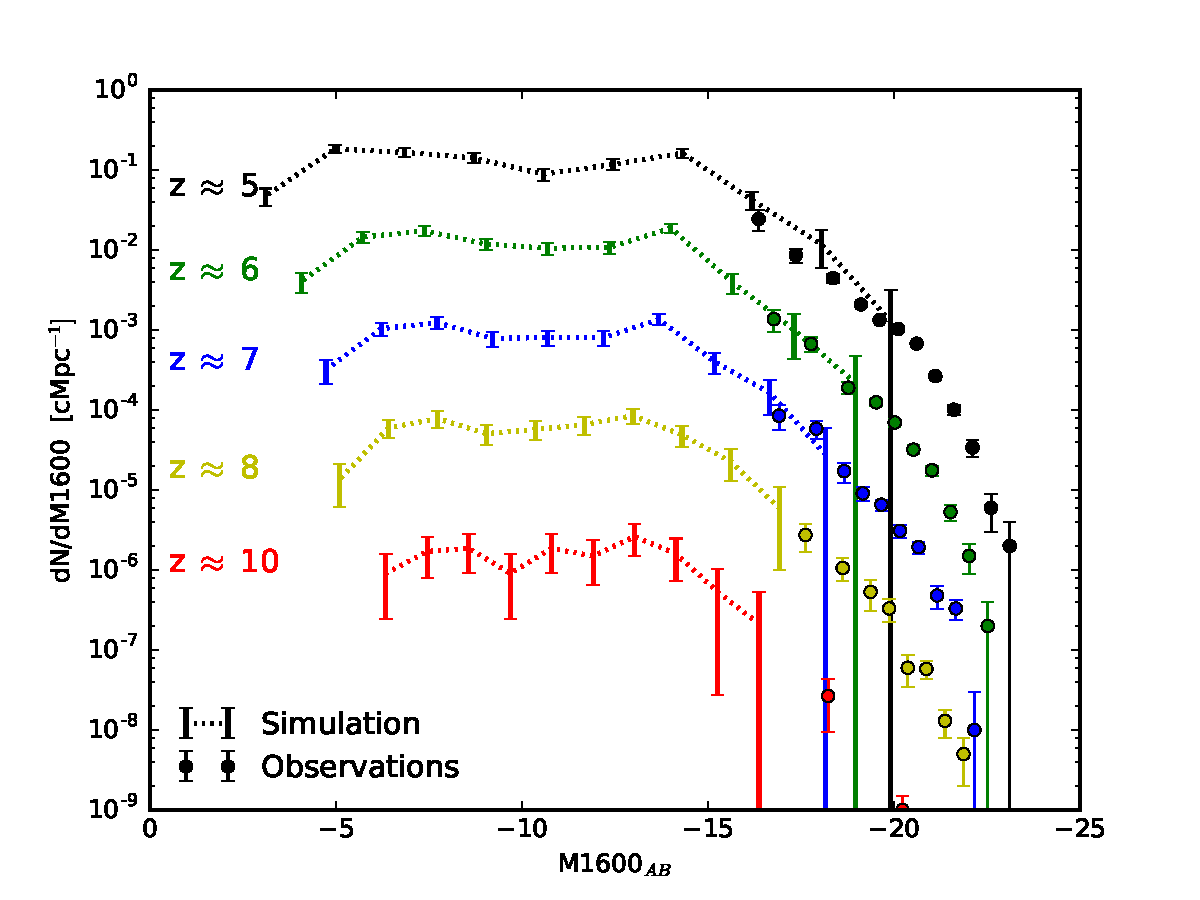
\includegraphics[width=.95\linewidth]{img/02/luminosity_function.pdf}
%        \caption{Fonction de luminosité dans la bande $M_{1600}$.
%}
% 		\label{fig:test_SFH}
%\end{figure}

%Des test plus poussés seront développés plus loin.

\clearpage
\section{La vie radiative}
\label{sec:etoilerad}

%\subsection{Vie}
%le diagram HR

Une fois le nuage de gaz effondré et les réactions thermonucléaires amorcées, l'étoile amorce sa séquence principale.
C'est la phase qui représente la majeure partie de la vie d'une étoile.
Elle consiste en un équilibre hydrostatique entre gravitation et pression interne, maintenue par les réactions de fusion nucléaire.
L'étoile va consommer son hydrogène pour résister à l'effondrement gravitationnel, il en résultera une formation d'hélium.
%develloper le cycle proton proton ?
L'équation simplifié du processus de fusion, appelé cycle proton-proton (PP) est :
\begin{equation}
4p \leftrightarrow He^4 + 2e^+ + 2\nu + E.
\end{equation}

Plus une étoile est grosse plus le taux de réaction doit être élevé pour lutter contre la gravité.
Il en résulte que les grosse étoiles sont plus énergétique, et émettent donc plus de rayonnement ionisant.
En contre partie, ce taux de réaction élevé mène à une durée de vie plus courte.
Du fait de leurs masses, les popIII, émettaient un fort rayonnement ionisant, et avaient une vie relativement courte.

%materiaux de base est l'hydrogene\\
%plasma donc hydrogène ionisé 


\subsection{Fonction de masse Initiale}

Les étoiles naissent en groupe, et toutes ne sont pas identique.
Pour caractériser cette diversité, il existe la notion de fonction de masse initiale (\ac{IMF}), qui exprime la probabilité de former une étoile d'une certaine masse dans un population.
Parmi les \ac{IMF} plus connues il y a :

\begin{itemize}
\item \cite{1955ApJ...121..161S}
\item \cite{1979ApJS...41..513M}
\item \cite{2001MNRAS.322..231K}
\item \cite{2003PASP..115..763C}
\end{itemize}

%TODO Quelles sont les différences

%Comme nous l'avons abordé plus haut, les étoiles de population III avaient tendance a être très massive.

Des travaux comme \cite{2003MNRAS.344L...7C} suggère que lors de la réionisation, il y avait formation d'une forte proportion d'étoile massive, j'ai donc utilisé par la suite une \ac{IMF} Top-Heavy.
%TOTO description top heavy

%: difficulté a reioniser avec Salpeter -> passage a top heavy -> justification 
%Fonction de masse IMF Top Heavy

\subsection{Starburst99}
\label{sec:staburst}
%Pour modeliser 
%paramètre d'entrée
%sorties

Une fois les étoiles formées, il est nécessaire de les faire rayonner.
Pour ce faire il faut, à partir de leurs masses et de leurs ages, calculer leurs émissivité.
Pour déterminer quel est le lien entre age, masse et luminosité d'une particule stellaire on utilisera un modèle de population stellaire.


Les étoiles d'une population ayant des masses et des évolutions différentes, l'émission résultante sera la somme des contributions individuelles.
La modélisation de population stellaire est complexe, et il existe différent modèles dédiés à cette tache.
On peut citer entre autres :

\begin{itemize}
\item Starburst99 \cite{leitherer_starburst99:_1999} 
\item \cite{2003MNRAS.344.1000B}
\item FSPS \cite{2009ApJ...699..486C}
\end{itemize}

A partir d'informations caractéristiques d'une population stellaire, comme sa masse, son \ac{IMF} ou sa métallicité, ces modèles retournent un spectre d'émission et son évolution en fonction du temps (cf Fig \ref{fig:spectre_starburst}).
Le choix a été fait d'utiliser Starburst99, car en plus des spectres, il retourne plusieurs informations utiles au modèle comme l'énergie et la masse injectées par les supernovae (section \ref{sec:sncali}).

\begin{figure}
        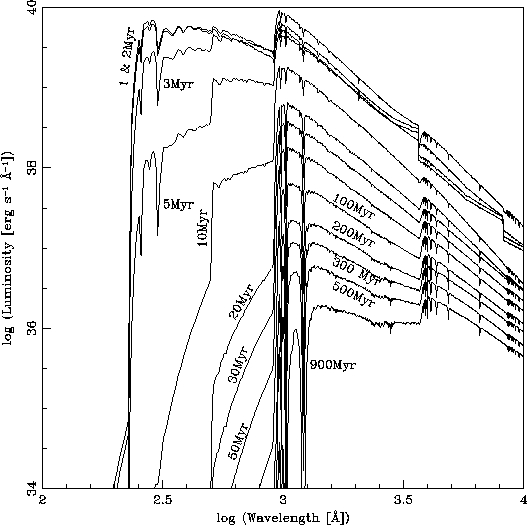
\includegraphics[width=.95\linewidth]{img/03/spectre_starburst.jpg} 
        \caption[Spectres Starburst99]{Spectre d'émission d'une population stellaire généré par Starburst99.
        Ici avec les paramètres sont $M_{pop}=10^6 M_\odot$, \ac{IMF} de Salpeter ($\alpha=2.35$ et intégration de 1 à 100 M$_\odot$ 
 		\label{fig:spectre_starburst}}
\end{figure}

%injection d'énergie dans le solveur radiatif, ok mais combien?\\
%calibration energetique et Starburst99\\

%J'ai commencé mes calibrations avec une \ac{IMF} de Salpeter, mais il s'est vite avéré que les sources n’émettaient pas assez de photons ionisant et que les boites n'arrivaient pas a reioniser.
%La majorité des simulations que j'ai réalisées ensuite utilisent une \ac{IMF} Top-Heavy.


A partir des spectres obtenus avec Starburst99 (cf section \ref{sec:staburst}), nous n'allons garder que la partie capable de ioniser l'hydrogène (toutes les longueurs d'onde plus courte que 912$\AA$) :

\begin{equation}
E_{ion (t)} = \int_{13.6eV}^{+\inf} h \nu_{(t)} d\nu
\end{equation}

En divisant l'énergie totale obtenue à partir de cette intégration, par l'énergie moyenne des photons obtenue à partir des spectres (cf section \ref{sec:groupedephotons}), on obtient l'évolution du flux de photons ionisant, présenté sur la figure \ref{fig:flux}.
\begin{figure}
        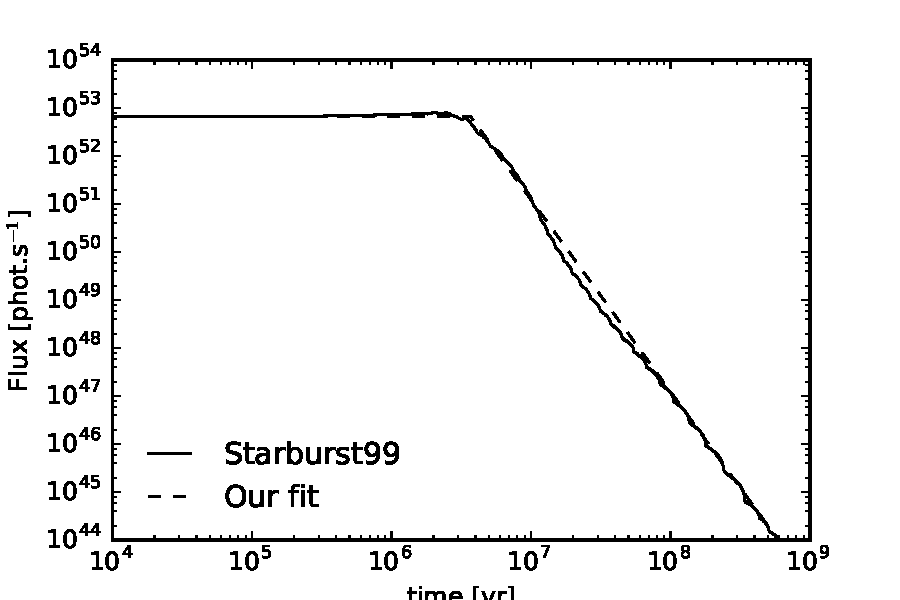
\includegraphics[width=.95\linewidth]{img/03/flux.pdf} 
        \caption[Émissivité ionisante]{Émissivité ionisante intégrée en fonction du temps.
        La population présente deux phases d'émission, une phases constante suivie d'une rapide décroissance.
 		\label{fig:flux}}
\end{figure}
Le profil obtenu présente un plateau d'émissivité constante suivie d'une rapide décroissance.
Ce profil peut être raisonnablement approximé par:

\begin{equation}
    S = 
\begin{cases}
    S_0 ,         & \text{if } t < t_{life}\\
    S_0.t^{-4},   & \text{if } t_{life} \leq t < 100t_{life} \\
    0,   & \text{if } 100t_{life} \leq t
\end{cases}
\end{equation}

où $t_{life}$ est définis comme étant l'age de la population au moment de changement de régime.
Par la suite nous utiliserons la valeur de $t_{life} = 3.7$Myrs.

Étant donné la rapide décroissance en luminosité, les étoiles sont arbitrairement éteintes après $100 \cdot t_{life}$.

Le flux obtenu correspond au flux d'une population de $10^6M_\odot$, et ces valeurs seront pondérées au prorata de la masse de la particule stellaire : une particule de $10^5M_\odot$ émettra  simplement 10 fois moins de photons ionisant qu'une population de $10^6 M_\odot$.

Cette émissivité sera ensuite pondérée par un paramètre d'efficacité.
Ce paramètre libre reflète l'impact d'une grande partie de la physique sous grille, sur le rayonnement.
En effet, nous ne résolvons pas certains processus, comme par exemple l'absorption par la poussière, qui va empêcher la radiation de sortir de l’environnement de la population.
Ce paramètre est analogue à une fraction d'échappement intrinsèque et ne doit pas être confondu avec la fraction d'échappement des galaxies que nous aborderons par la suite (voir section \ref{sec:fesc}).

Il nous reste encore à caractériser le type de photons à émettre.
La gestion des groupes de photons a été abordée dans la section \ref{sec:groupedephotons}, nous ne travaillerons par la suite qu'en émission mono-groupe.
Les caractéristiques des photons émis dans le cas d'une \ac{IMF} Top-Heavy sont présentés sur la table \ref{tab_photon}.

\begin{table}
\begin{tabular}{l l }
	$<h\nu>$	&  $23.42$ eV \\
	$\alpha_e$	&  $2.35.10^{-22}$ m$^2$ \\
	$\alpha_i$	&  $1.82.10^{-22}$ m$^2$ \\
\end{tabular}
\caption[Propriété des photons]{Propriété des photons émis par les sources.
Ces valeurs ont été calculées à partir des spectres obtenus avec Starburst99.
\label{tab_photon}}
\end{table}


En pratique, il faudra calculer l'émissivité sur toute la grille.
Cette opération est simplifiée par l'utilisation de la liste chaînée de particule (cf section \ref{s}).
En effet, on passera en revue toutes les cellules, et pour chaque cellules on passera en revue toutes ses particules.
On testera alors si une particules est une étoiles (la liste chaînée contient également les particules de matière noire), et si cette étoiles est dans un stade où elle émet de l'énergie lumineuse.
Si c'est le cas, on calculera son émissivité et on injectera cette énergie sous forme de source dans l'équation \ref{eq:densite_energie}.
Le calcul de $\dot{N}_\nu^*$ sera effectué dans toutes les cellules.


%TODO intégration de l'énergie et de la section efficace


%We found a mean energy of $<h\nu> = 23.42$ eV,
%an energy weighted cross section of
%$\alpha_e = 2.35.10^{-22}$ m$^2$
%and a number weighted cross section of
%$\alpha_i = 1.82.10^{-22}$ m$^2$


%Masse de la population\\
%produit en croix pour correspondre a la masse dans simu\\
%integration seulement sur energy ionisante\\
%
%Multigroupe frequence\\
%multigroup temporel\\



%\section{Le problème de la masse des étoiles}
%
%%le paramètre de masse des étoiles change la reionization\\
%%effet numérique\\
%%le rayonnement est piégé dans les cellules\\
%
%Durant mes calibrations, il s'est avéré que le paramètre de résolution de la masse des particules stellaire avait une grande importance dans l'évolution de la fraction ionisée.
%Même si celui ci n'a pas d'impact sur la SFR globale, le taux d'ionisation moyen est fortement dépendant de ce paramètre (cf Fig .\ref{fig:mstar}).
%Plus la résolution stellaire est élevée, plus la boite réionise tard.
%Les "grosse" particules stéllaire mènent a un taux d'ionisation plus important.
%
%\begin{figure}[bth]
%        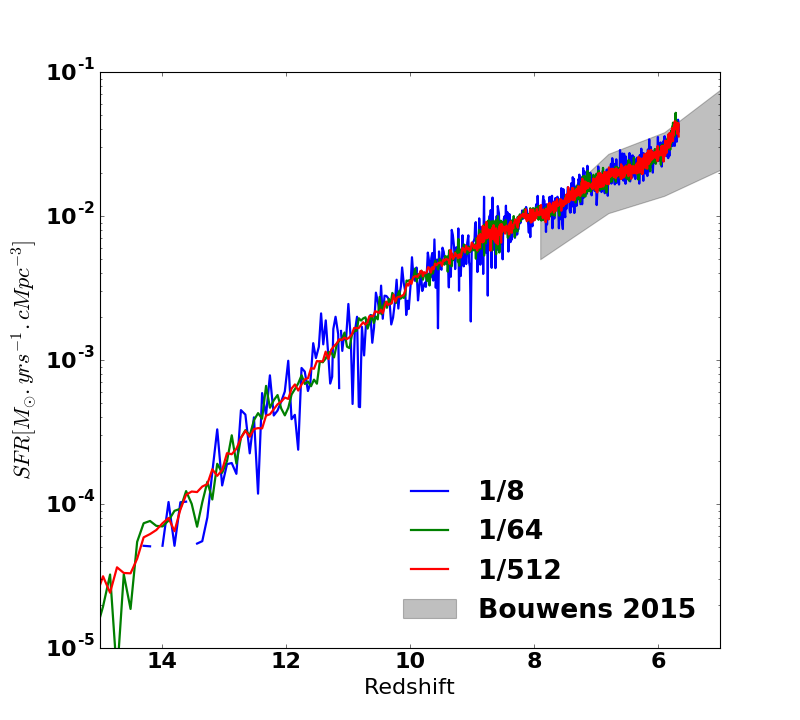
\includegraphics[width=.45\linewidth]{img/02/Mstar_SFH.png} 
%        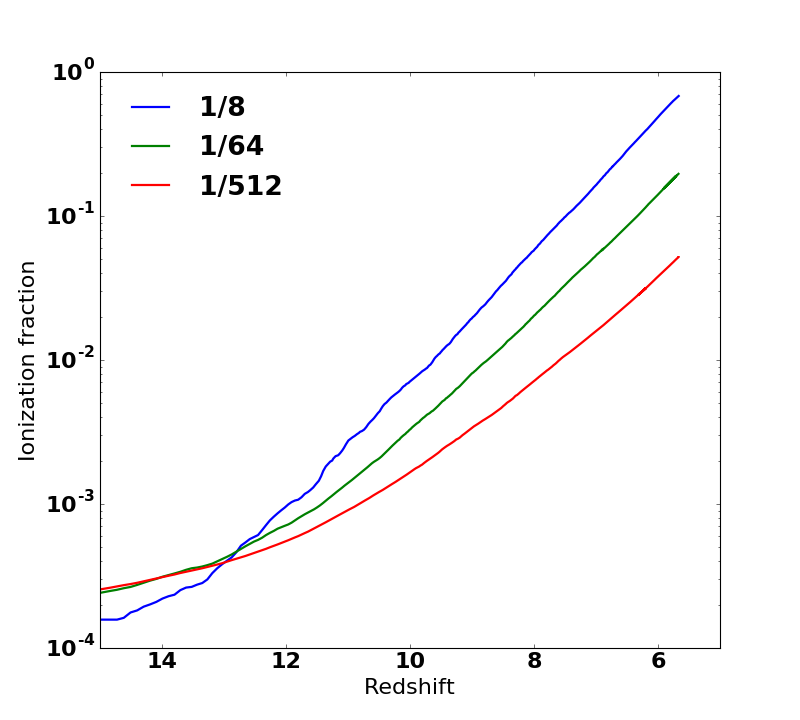
\includegraphics[width=.45\linewidth]{img/02/Mstar_xion.png} 
%        \caption{
%        En changeant le parametre de résolution en masse des particules stellaire, la SFH moyenne reste constante mais l'histoire d'ionisation s'en trouve impacté.
%}
% 		\label{fig:mstar}
%\end{figure}

